\documentclass[a4paper,12pt]{report}

\label{PACOTES}
%\usepackage[acronym,translate=true]{glossaries}
%\makeglossaries
\usepackage[utf8x]{inputenc}         % acentos
\usepackage[portuges,brazil]{babel} % traduz titulos,sections


\usepackage{graphicx}
\usepackage{fancyvrb}
\usepackage{float}
\usepackage{tikz}
\usepackage{multirow}
 
\label{MACROS}
\DefineVerbatimEnvironment{verbatim}{Verbatim}{xrightmargin=.1in}

\label{DEF}
\def\checkmark{\tikz\fill[scale=0.4](0,.35) -- (.25,0) -- (1,.7) -- (.25,.15) -- cycle;}
\graphicspath{{./figs/}}

% Title Page
\title{ Relatório: Mormodo Verde }
\author{Bruno Granato \\
	Nicholas Quagliani\\
	Renata Baptista\\
	Vinicius Mesquita}

%\institute{
%	Orientador: <nome-do-orientador>\\
%	Co-orientador: <nome-do-co-orientador> \\ [1 ex]
%	<nome-instituto>
%}
\begin{document}
\maketitle


\tableofcontents
\chapter{Introdução}
	\section{Motivação}
		Dado a correria imposta pelas atividades diárias e viagens ocasionais, é comum que as plantas domésticas fiquem neglicenciadas. Para evitar isso e permitir a hidratação e a quantidade de luminosidade necessárias, foi concebido o Mordomo verde, que é um sistema para o cuidado das plantas.
	\section{Objetivo}
		Este projeto tem por objetivo a construção de um sistema que regue e controle a quantidade de luz solar recebida por plantas, uma vez sabido a espécie da mesma.
		
		A ideia é interagir com o usuário por meio de um \textit{display} LCD e botões do mesmo módulo, para que ele possa determinar qual é a espécie da planta, entre as pré-determinadas. 
		
		Além disso, haverá o sensoriamento do ambiente. Colhendo informações de temperatura, umidade e luminosidade.
		
		De posse de ambas as informações, o microcontrolador usará uma relação biológica para decidir a quantidade de água e a inclinação das persianas necessária. 
		
		Assim, o microcontrolador agirá nos atuadores fazendo com que as necessidades das plantas sejam supridas. Neste projeto, o sistema será implementado para duas plantas diferentes.
	\section{Organização do Documento}

\chapter{Tecnologias Utilizadas}
	\section{Especificações}
	
	\subsection{Plantas}
	Duas plantas de espécies diferentes foram utilizadas durante o desenvolvimento do projeto. A renda-portuguesa (\textit{Davallia fejeensis}), Figura~\ref{fig:renda}, é uma planta nativa da ilhas Fiji, que se desenvolve melhor em ambientes iluminados, porém sem sol direto, que pode ser cultivada no interior de apartamentos, no chão ou em local baixo, perto da janela. Uma vez que a renda-portuguesa também não deve ficar exposta ao vento, pois é frágil. Ela deve ser regada, em dias quentes, ou seja, temperaturas acima dos 30$\textdegree$~C, todos os dias; quando abaixo disso, de dois em dois dias. Mas sempre é recomendado verificar a umidade do solo, a fim de certifica-se que o mesmo se encontra devidamente úmido. Discussões sobre a quantificação desses valores serão discutidos na seção %ref da seção \ref{sec:q}%.
		
\begin{figure}[!h]
	\centering
	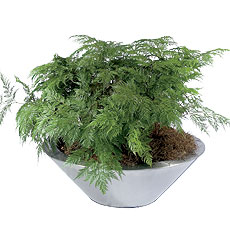
\includegraphics[width=0.4\linewidth]{figs/renda}
	\caption{Exemplar de renda-portuguesa.}
	\label{fig:renda}
\end{figure}

	A segunda planta adquirida foi uma avenca (\textit{Adiantum capillus-veneris}), que pode ser vista na Figura~\ref{fig:avenca}. Ela precisa de um ambiente úmido, quente e de luminosidade indireta, com esses ingredientes ela é capaz de se desenvolver de forma saudável. Assim como a renda-portuguesa, ela não deve receber vento diretamente. Como a umidade é um ponto-chave para seu desenvolvimento, deve-se verificar que a mesma mantenha uma umidade do solo maior que quando comparado com a planta anterior. Logo, em um tempo quente ela deve ser regada mais constantemente. Com essas características, a avenca também pode se desenvolver bem em um ambiente como um apartamento, o que torna a dupla de exemplares escolhida muito boa para o nosso projeto. 
	
	 
\begin{figure}[!h]
	\centering
	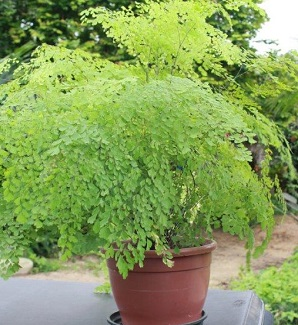
\includegraphics[width=0.4\linewidth]{figs/avenca}
	\caption{A avenca, (\textit{Adiantum capillus-veneris}).}
	\label{fig:avenca}
\end{figure}
	
	\section{Projeto de Hardware}
	
		\subsection{Sensor de temperatura - LM35}
		
		Sensor de precisão de temperatura centígrado, apresenta uma saída em tensão linearmente proporcional a graus Celsius. Além disso, não necessita de nenhuma calibração externa.
		
		Dentre suas especificações, ressaltamos, a sua acurácia de 0.5$\textdegree$ (a +25$\textdegree$ Celsius), suficiente para aplicação. Além disso, sensor é capaz de medir temperaturas de -50$\textdegree$ a 150$\textdegree$ Celsius, o que cobre a faixa dinâmica de trabalho no projeto. Apesar disso, usaremos o sensor na configuração básica conforme a Figura 2.1 Consideramos também a faixa de tensão de trabalho que é de 4~V a 30~V, o que permite a alimentação com a placa escolhida e drena menos de 60~$\mu$A, também dentro da capacidade da placa.
		\begin{figure}[!htb]
			\centering
			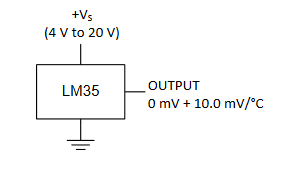
\includegraphics{LM35_config_basica}
			\caption{Diagrama do LM35 na configuração básica}
			\label{Rotulo}
		\end{figure}
		\subsection{Sensor de umidade do Solo Higrômetro}
		Sensor é capaz de perceber variações da umidade do solo, tem saída em volts que é linearmente depende da umidade.
		Trabalha com tensão de Operação: 3, 3 - 5 V, o que torna viável sua utilização com o Arduino. Tem saída digital em LED, com a sensibilidade calibrada por potenciômetro. Mas essa função não será utilizada no projeto.
	
		\subsection{Sensor de luminosidade LDR 5mm}
		
		Sensor de Luminosidade LDR de 5~mm de diâmetro. Este altera a resistência em seus terminais conforme a luminosidade que é submetido.
		
		Especificações:
		Resistência quando há luz :~1~k$\Omega$.
		
		Resistência no escuro :~10~k$\Omega$.
		
		Tensão máxima:~150~V.
		
		Potência máxima:~100~mW.
		
		\subsection{Plataforma Arduino - Mega}	
		\subsection{Mecânica}
			Para fazer o controle da água que cai sobre as plantas, foram utilizadas válvulas solenoides. São dispositivos que funcionam como torneiras controladas por um sinal elétrico. O momento correto para regar a planta é determinado pelo Arduino, baseado nos dados obtidos pelos sensores. Quando for necessário, o sistema aciona uma relé que permite que a válvula receba o sinal elétrico que realizará sua abertura, fazendo as plantas serem molhadas.	
			
			\begin{figure}[!htb]
				\centering
				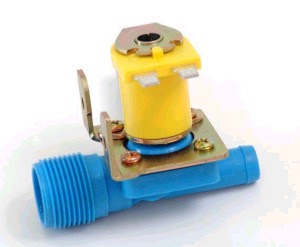
\includegraphics{valvula}
				\caption{Válvula solenoide}
				\label{Rotulo}
			\end{figure}
		
			O controle da luminosidade sobre as plantas é realizado através de um servo instalado no eixo de um sistema de persianas. Dependendo do dado obtido pelo LDR, o Arduino faz com que o servo gire mais ou menos, variando a inclinação das persianas e adequando a luminosidade à planta em questão. FALTA FALAR SOBRE QUAL SERVO VAMOS USAR""
		
	\section{Projeto de software}
	Primeiro, era necessário colher os dados dos sensores, lendo suas respectivas entradas analógicas. Devido a maneira que o arduino faz essas leituras, foi necessário adicionar um delay entre as aquisições para que o microcontrolador tivesse tempo o suficiente para chavear as entradas analógicas com seu único conversor A/D.
	
	De posse dessas informações e da informação do tipo de planta que tem no slot, foi possível controlar os atuadores para regar a planta e fornecer mais ou menos luminosidade.
		
\chapter{Implementação}

\section{Montagem da estrutura}
A estrutura do projeto foi feita com canos PVC, pelo custo e resistência a água do material. Os sensores foram presos a uma plataforma de plásticos para facilitar o manuseio do usuário final. Por fim, o Arduino e suas ligações foram colocadas em uma caixa, a qual tem foi preso o display LCD com os botões, para evitar danos a parte elétrica.

A ideia inicial era fazer uma estrutura retangular e prender a persiana por cima como no modelo abaixo COLOQUEM A FIGURA DO MODELO PQ NINGUEM POS AS FOTOS E ETC QND EU PEDI.
Contudo, durante a execução do projeto, como já tinha sido avaliado, constatamos que a inclinação de 90º não era suficiente para o funcionamento ideal dos sistemas de persianas.

A solução encontrada foi aumentar a angulação, gerando a estrutura final como na figura abaixo COLOQUEM A FIGURA ABAIXO.


\chapter{Conclusões}

 
 
\addcontentsline{toc}{chapter}{Bibliografia}
\bibliographystyle{coppe}
\bibliography{My_Collection_used}	
	
	
	
	
	
	
	
	
	
	
	
		
	
	
	

\end{document}          
